\chapter{Radar system firmware development}\label{sec:radar-system-firmware-development}
The main objective of the system is the replacement of the high-cost, deferred sampling analogue-to-digital converter (ADC) with a microcontroller unit (MCU) capable of processing the signals in real-time and transmitting the useful information to a receiving device using a Bluetooth Low Energy (BLE) link.

For that purpose, an MCU has been selected according to selection criteria detailed in Chapter 2 and a firmware has been developed and tested. This firmware is executed in the embedded MCU integrated in the MCU PCB, described in Chapter 4. % TODO: Section ZZZ
The firmware is made up of software which controls embedded hardware in the MCU package and carries out processing of the incoming signals.

The system firmware function is three-fold. First, it is responsible of configuring and handling the operation of the peripherals of the system, which enable the interaction with system elements found in different parts of the system. Secondly, it also provides the digital signal processing (DSP) needed to process the incoming data sampled from the ramp signals. Finally, it prepares the processed data to be sent wirelessly to a receiving device and handles this wireless communication.

The integrated peripherals are configured using low-level registers in the MCU [REF] and the routines for the DSP are programmed in the source code. The source code is written in the C programming language with some parts optimised with ARM assembly (ASM) instructions. These ASM instructions are low level code that is executed by the MCU. Having some parts developed directly in ASM, the control is much greater and lower level, allowing for more optimisations of the firmware in specific parts.

The developed firmware is split into two parts, which are programmed and executed in two different central processing units (CPU) embedded into the same MCU:
\begin{itemize}
	\item The main processor, an ARM Cortex-M4 [REF] which handles digital signal processing (DSP) of the incoming radar signals.
	\item The secondary processor, an ARM Cortex-M0+ [REF] which acts as a wireless co-processor handling the wireless communication.
\end{itemize}

This dual processor architecture is provided by the manufacturer of the MCU and enables the wireless communication stack to handle the BLE transmission without interrupting the data acquisition and DSP performed by the main processor. This is due to the fact that instructions related with the processing of sampled data can run in one processor while the execution of the wireless stack can run in the secondary processor at the same time. This pipeline parallelisation architecture is a key factor in allowing the real-time function of the system. A high-level diagram showing the overview of the firmware architecture is shown in \cref{fig:firmware_overview}.

\begin{figure}[ht]
	\centering
	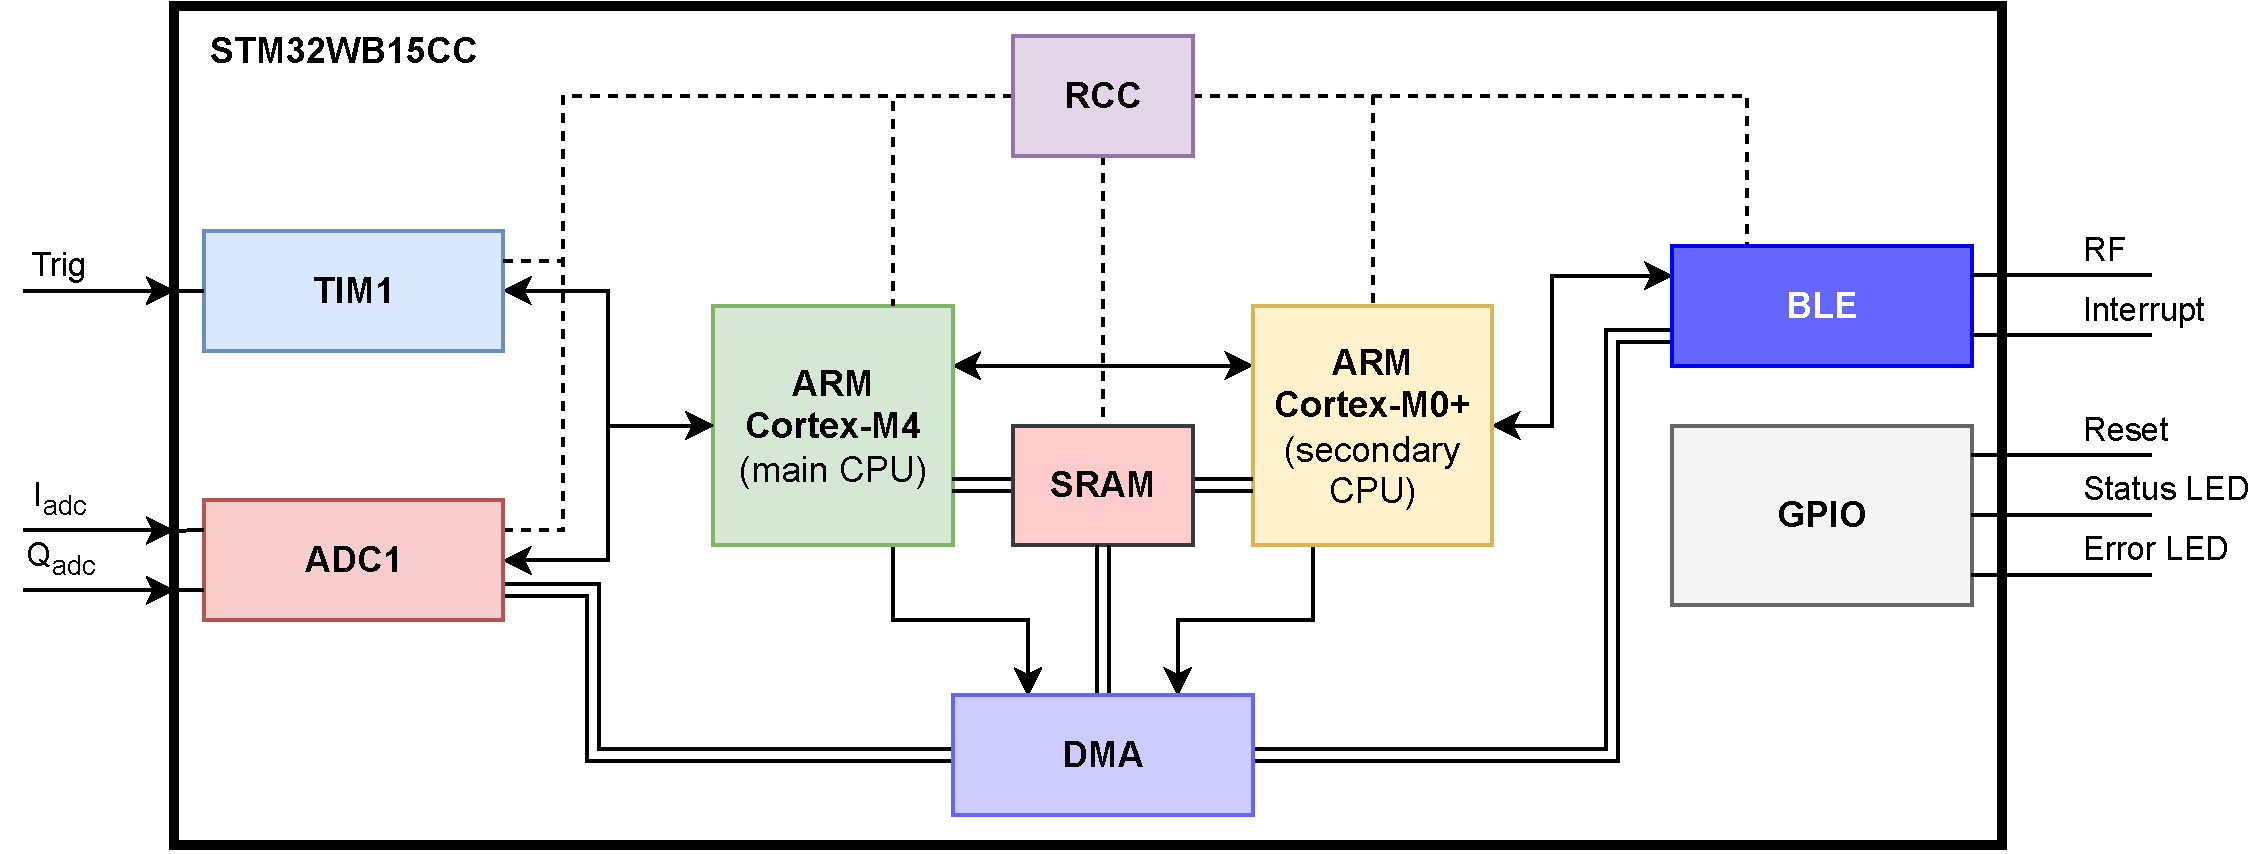
\includegraphics[width=\linewidth]{firmware/firmware_overview}
	\caption{Firmware and hardware architecture overview. Dotted lines represent clock lines, double lines represent data bus and uni or bidirectional arrows represent instruction flow. TIM1 is the Timer 1 used to trigger the sampling of the ADC, which initiates on a ramp trigger signal coming from the radar. ADC1 is the ADC that samples the $I_{\mathrm{adc}}$ and $Q_{\mathrm{adc}}$ signals coming from the IF stage. SRAM is the system memory. BLE is the hardware that handles RF communication. The DMA controls the transfer of data from devices to memory and between devices. GPIO controls the general IO of LEDs and a button}
	\label{fig:firmware_overview}
\end{figure}

In this chapter the developed firmware is described, outlining the software design decisions that have been taken and the reasoning behind them. Additionally, the interaction between the MCU peripherals and the firmware is explained. Finally, the description of the wireless stack and its role in the system is carried out.

\section{Digital Signal Processing (DSP)}

In this section, the firmware part devoted to the processing of the incoming conditioned signals is described. Itself, the DSP firmware contains two parts corresponding to the two operating modes of the transmission: the primary mode, based on computing the fast Fourier transform (FFT) and a secondary mode which additionally sums the frequency bins obtained from the FFT. In this section, the peripherals involved are described. The processing of ramp data by the DSP routines constitutes the DSP pipeline of the system. A temporal diagram showing the DSP process and peripherals is shown in \cref{fig:firmware_dsp_overview}.

\begin{figure}[ht]
	\centering
	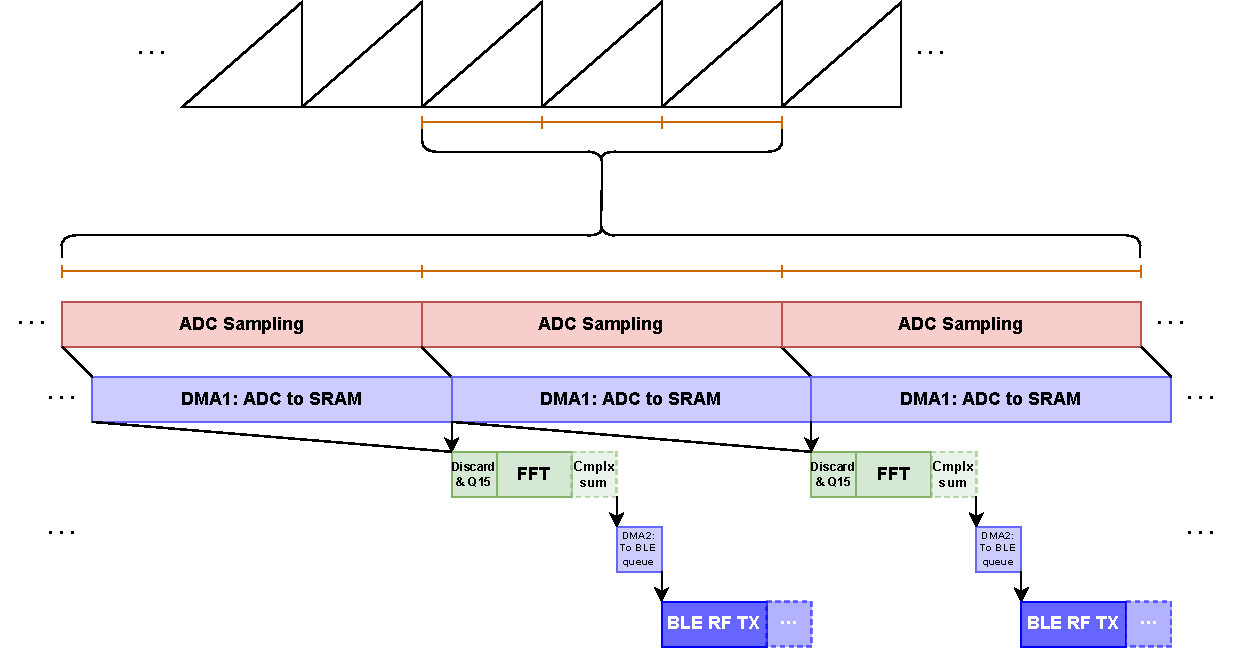
\includegraphics[width=\linewidth]{firmware/firmware_dsp_overview}
	\caption{DSP routines temporal overview. Note that due to the asynchronous nature of the ADC sampling and DMA controller, the samples from a previous ramp are processed and transmitted during the next one. This allows the system to work in real time. The downward arrows represent interrupts coming from one process or peripheral to another. For instance, when the DMA controller finishes transferring the samples of a ramp to memory, the DSP routines start executing. The green boxes represent the DSP routines: Preprocess includes the sample discard and the Q15 format conversion. Dashed boxes represent optional or variable stages.}
	\label{fig:firmware_dsp_overview}
\end{figure}

\subsection{MCU peripherals}

The STM32WB15CC microcontroller unit (MCU) integrates several peripherals useful for the purpose of signal digitisation and processing. These peripherals must be configured by the firmware prior to performing the DSP routines. The following peripherals are used in this part of the firmware:
\begin{itemize}
	\item Reset and clock controller (RCC) that configures the clock frequency of the peripherals and the MCU. This is configured to the maximum possible clock frequency that the MCU allows of \SI{64}{\mega\hertz}. The maximum clock frecuency is chosen so that the processor can execute each instruction in a shorter time.
	\item 10-channel 12-bit analogue-to-digital converter (ADC) of which two channels are used, connected to the incoming intermediate (IF) frequency signals $I_{\mathrm{adc}}$ and $Q_{\mathrm{adc}}$. As outlined in Section 2 % TODO: Section ZZZ
	, this ADC can have a maximum sampling rate of \SI{2.5}{MSps}.
	\item Configurable timers, used to discipline the ADCs' sampling. They are trig\-gered by the external ramp trigger signal \textit{Trig} coming from the radar.
	\item Direct memory access (DMA) peripheral, used for memory transfers to and from peripherals and the MCU integrated static random-access memory (SRAM) without interrupting the firmware execution in the main CPU.
	\item General purpose input/output pins (GPIO) used for reset button, indication LEDs and the external ramp trigger signal \textit{Trig} coming from the radar.
\end{itemize}

These peripherals work in conjunction with the software DSP to obtain the data to be sent via the wireless BLE link. The configuration of these peripherals performed in the firmware source code can be found in Appendix ZZZ.

\subsubsection{Reset and clock controller (RCC) configuration} \label{sec:rcc}

The reset and clock controller (RCC) handles the clock frequency configuration of the different parts of the system. All the clocks of the system are derived from a source external master clock of \SI{32}{\mega\hertz} and thus synchronised to it. The clock network tree can be seen in \cref{fig:firmware_clock_tree}. The clock frequencies are configured as follows:
\begin{itemize}
	\item External master clock: High-speed external (HSE) oscillator of \SI{32}{\mega\hertz}.
	\item Main CPU: configurable between \SI{100}{\hertz} and \SI{64}{\mega\hertz}. The selected configuration is the maximum value of \SI{64}{\mega\hertz}.
	\item Secondary CPU (BLE stack): configurable between \SI{100}{\hertz} and \SI{32}{\mega\hertz}. The selected configuration is the maximum value of \SI{32}{\mega\hertz}.
	\item SRAM: configurable frequency range identical to Main CPU. The selected configuration is the maximum value of \SI{64}{\mega\hertz}.
	\item Timer: configurable frequency range identical to Main CPU. The selected configuration is the maximum value of \SI{64}{\mega\hertz}, it is synchronised to the Main CPU clock.
	\item MCU ADC: configurable between \SI{0.5}{\hertz} and \SI{32}{\mega\hertz}. The selected configuration is the maximum value of \SI{32}{\mega\hertz}, it is synchronised to the Main CPU clock.
\end{itemize}

The other clocks of the system are left to the default value or are automatically configured depending on these clocks. They are used for internal caches of the processors or controlling the switched power supply, for instance.

\begin{figure}[ht]
	\centering
	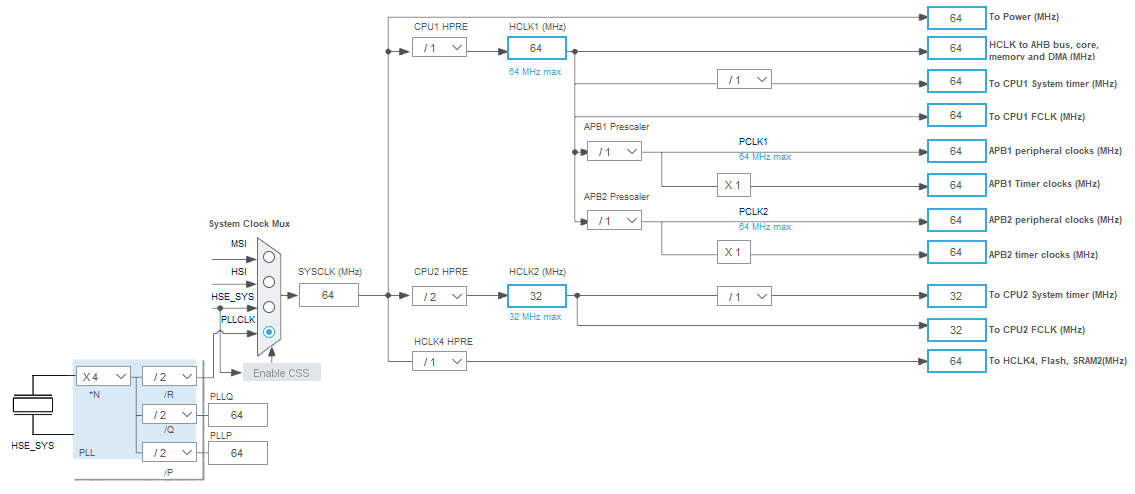
\includegraphics[width=\linewidth]{firmware/firmware_clocks}
	\caption{Clock tree of the peripherals and CPUs of the system. The high speed external (HSE) oscillator is a \SI{32}{\mega\hertz} crystal. Only the relevant clocks are shown, as the rest of the clocks are configured by default or automatically}
	\label{fig:firmware_clock_tree}
\end{figure}

\subsubsection{Analogue-to-digital converter 1 (ADC1) and Timer 1 (TIM1) configuration} \label{sec:adc_tim_config_v_vector}

The integrated analogue-to-digital converter (ADC1) is configured based on the frequency characteristics of the incoming intermediate frequency (IF) signals. The minimum sampling rate requirement outlined in Section 2 determines the sampling rate of the ADC. This ADC sampling rate can have a maximum of \SI{2.5}{MSps} when a \SI{35}{\mega\hertz} clock is supplied to it. Nonetheless, this clock frequency can only be achieved when the ADC is free-running and not synchronised to the master clock. The ADC needs to be synchronised to the master clock to be synchronised to the system operation. In this scenario, the maximum clock frequency that can be supplied to the ADC is of \SI{32}{\mega\hertz}.

The ADCs are configured to perform a sequential sampling of the channels $I_{\mathrm{adc}}$ and $Q_{\mathrm{adc}}$. The clock frequency of the ADC is set to  \SI{32}{\mega\hertz} according to \cref{sec:rcc}. However, the triggering of the signal is done by Timer 1 (TIM1). Effectively, the clock frequency supplied to the ADC is much higher than the triggering signal frequency coming from Timer 1. This configuration of different ``working'' and ``triggering'' clocks is used to allow the user to configure the ADC sampling rate on the fly, without needing to reconfigure the clock tree, which involves a system reset. As the ADC is a successive approximation register (SAR) ADC, the maximum sampling rate of the ADC is given by the total sample conversion time $t_\mathrm{CONV}$ such that $f_s = 1/t_\mathrm{CONV}$. $t_\mathrm{CONV}$ depends both on a predefined sampling time $t_\mathrm{S}$ and the sample successive approximation time $t_\mathrm{SAR}$. These two times are factory set by the manufacturer: $t_\mathrm{S}$ has a minimum value of 1.5 ADC clock cycles and the approximation time is a fixed value of 12.5 ADC clock cycles \cite[p.~104]{STMicroelectronics2022}.
By configuring the ADC clock to \SI{32}{\mega\hertz}, the maximum sampling rate of the ADC can be obtained as follows:
\begin{align}
	t_\mathrm{S} = \frac{1.5}{f_\mathrm{ADC}} &= \SI{46.875}{\nano\second}\\
	t_\mathrm{SAR} = \frac{12.5}{f_\mathrm{ADC}}
	&= \SI{390.625}{\nano\second}\\
	t_\mathrm{CONV} = t_\mathrm{S} + t_\mathrm{SAR} &= \SI{437.482}{\nano\second}\\
	f_{s,\max} = \frac{1}{t_\mathrm{CONV}} &= \SI{2.286}{MSps}
\end{align}
As the ADC input channels are sampled sequentially, the maximum sampling rate per channel is $f_{s,\max}/N$ with $N$ being the number of channels. For this system case, as they are two channels to be sampled $I_{\mathrm{adc}}$ and $Q_{\mathrm{adc}}$, the maximum sampling frequency per channel is \SI{1.143}{MSps}.

To enable the user to sample at a lower frequency, the ADC running clock is left to the maximum value (\SI{1.143}{MSps}) but the sample clock (the clock of the sampling trigger signal) is provided by Timer 1 and configurable by the user.

The sampling clock is provided by an external trigger generated by TIM1. For this purpose, TIM1 is configured to produce this signal with the frequency $f_{s}$ desired. This frequency can be easily adjusted by the user of the system and is computed as follows:
\begin{equation}
	f_s = 2 f_{s,\mathrm{ch}}
\end{equation}

Where $f_{s,\mathrm{ch}}$ is the sampling frequency necessary to sample I or Q.

Moreover, TIM1's start itself is triggered by the external ramp trigger signal \textit{Trig} coming from the radar.

The ADC samples are extracted to a vector $\mathbf{v}$ in SRAM memory. Given the vector $\mathbf{v}$ of length $n$ denoted as:
\begin{equation}
 \mathbf{v} = (v_0, v_1, ..., v_{n-1})
\end{equation}

The vector size can be easily adjusted and is computed as follows:
\begin{equation}
	n = \lceil f_s T_c \rceil
\end{equation}

Where $f_s$ is the ADC sampling frequency previously defined.

\subsubsection{Direct memory access (DMA) configuration} \label{sec:dma}

The direct memory access (DMA) peripheral is used to transfer data in memory in two different parts of the system. The DMA features 8 independent channels that handle up to 8 concurrent memory transfers in the system [REF]:
\begin{itemize}
	\item In the acquisition phase (i.e. when the ADC samples), the DMA uses Channel 1 to transfer the ADC samples to the vector $\mathbf{v}$ in SRAM.
	\item In the data transmission phase (i.e. when the wireless transmission takes place), the DMA uses Channel 2 to transfer the DSP processed data to the memory used by the wireless co-processor. This latter operation is detailed in \cref{sec:data_transmission}.
\end{itemize}

This peripheral is capable to handle large memory transfers in parallel to the operation of the CPUs, which enable asynchronous transfer of data.

The DMA controller stores in $\mathbf{v}$ the samples that are generated in the ADC. The samples are stored in a channel-alternating increasing order, as shown in \cref{fig:firmware_adc_dma_vector}.

\begin{figure}[ht]
	\centering
	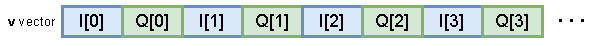
\includegraphics[width=\linewidth]{firmware/firmware_adc_dma_vector}
	\caption{Memory layout of ADC samples after DMA storage from ADC result to SRAM. Note the increasing and alternating order of channels. This layout facilitates the application of the FFT algorithm. Each sample value is of 12 bits and stored in a 16 bit unsigned integer due to the fact that variable sizes in bits must be a multiple of 8. In this particular case, as 12 bits is not a multiple of 8, the next available size is 16 bits. The values stored in the vector correspond to individual samples of a ramp.}
	\label{fig:firmware_adc_dma_vector}
\end{figure}

The ADC automatically finishes the data transfer when the buffer is full. This condition is reached when a ramp has ended as all samples from the ramp have been stored in the vector. When the data transfer is finished and the samples corresponding to one ramp are stored in $\mathbf{v}$, an interrupt is generated. This interrupt triggers the start of the DSP routines, as shown in \cref{fig:firmware_dsp_overview}.

The combined operation of the DMA, ADC1 and TIM1 peripheral constitute the data acquisition pipeline of the system.

\subsubsection{General purpose input/output (GPIO) configuration}

Some pins of the microcontroller have been configured as a general purpose input/output pin. In particular, the GPIO pins configured by the system are the following:
\begin{itemize}
	\item A pin for system reset button, which reboots the firmware when pressed.
	\item Two pins for function status LEDs, one LED lights up briefly whenever a ramp has finished sampling and another LED is used as an error status indicator.
	\item One test pin to wire any interrupt output to an oscilloscope for debugging purposes.
	\item A pin for the input of the external ramp trigger signal \textit{Trig} coming from the radar, this signal is tied to TIM1 start interrupt.
\end{itemize}

A diagram of the GPIO configurations in the pins of the MCU package is shown in \cref{fig:firmware_gpio}.



%The firmware includes a configuration routine at the start that discards every other trigger coming from the radar, this is due to the current radar node outputting two triggers, both at the start and end of the ramps. As the triggers that must be used is only the start of the ramp triggers, the other triggers must be discarded. This configuration is modifiable by the user if a radar node with only ramp start triggers is used.

\begin{figure}[ht]
	\centering
	\includegraphics[width=\linewidth, draft]{example-image}
	\caption{Outline of the MCU pin connections. The connections are classified as such: \textit{TRIG} is the trigger signal from the radar, \textit{IADC} and \textit{QADC} are the I and Q signals from the IF stage. \textit{RF} is the connection to the antenna. \textit{LED\_ERROR} and \textit{LED\_STATUS} are the output LEDs and \textit{RST} is the reset button}
	\label{fig:firmware_gpio}
\end{figure}

Additional details of the configuration of the GPIO pins can be found in Appendix E. % TODO: Appendix ZZZ

\subsection{DSP routines} \label{sec:dsp_routines}

The DSP pipeline is divided into four stages: outlying samples discard, sample normalisation and conversion to fixed point format, fast Fourier transform (FFT) computation and an additional optional stage of frequency bins summation, as shown in \cref{fig:firmware_dsp_chain}. These stages are implemented as functions or routines in the firmware source code. Moreover, to minimise memory utilisation every routine operates with the data in-place, i.e. computations modify the data in vector $\mathbf{v}$ without copying the data to another memory location. This approach reduces the use of excessive memory by preventing the creation of a new vector for every routine in the DSP chain. In this section the different DSP stages and the processing performed to sampled data is described.

\begin{figure}[ht]
	\centering
	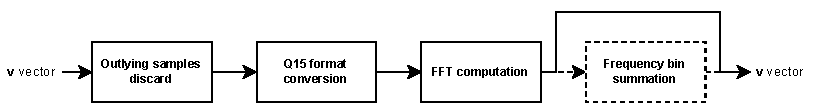
\includegraphics[width=\linewidth]{firmware/firmware_dsp_chain}
	\caption{DSP routines chain. The FFT bin summation is only available in the secondary operation mode. All other steps are common to both operating modes. The modifications are done in-place in the $\mathbf{v}$ vector}
	\label{fig:firmware_dsp_chain}
\end{figure}

\subsubsection{Outlying samples discard}

As commented in Section 2, for every ramp there exists a rising ramp and a dual ramp. Also, there is a short period of time at the beginning of the rising ramp where the phase-locked loop (PLL) of the voltage-controlled oscillator (VCO) is not locked. The useful samples from the intermediate frequency (IF) signal are present during the time the PLL is locked in the rising ramp. Therefore, the useless samples are discarded from the IF signal. The amount of samples discarded can be adjusted independently for each end of the ramps or set to zero. The routine operates on $\mathbf{v}$ as follows:
\begin{equation}
	\mathbf{v'} = [v_{r}, v_{r+1}, ..., v_{s-1}, 0, ..., 0] \qquad r = N_F,\ s= n- (N_F+N_L)
\end{equation}

Being $N_F$ the integer number of first samples to discard and $N_L$ the integer number of last samples to discard. Effectively, this routine zeroes $N_F$ and $N_L$ samples in the respective ends depending on the number of samples that are configured to be discarded. % TODO: A diagram showing the discard operation on the vector of samples is shown in Figure ZZZ.



\subsubsection{Sample normalisation and conversion to fixed point format}

In order to accelerate the computations for the FFT that are carried in a later routine, the samples are converted to a \textit{Q15} fixed point format [REF]. The \textit{Q notation} to denote fixed point formats is well known and used in the embedded DSP applications [REF2].

The \textit{Q15} format treats 16-bit unsigned integers as a signed fractional number of 1 bit for sign and 15 bits for the fractional part. The sign bit is the most significant bit (MSB). The range of this representation is $[-1, 1-2^{-15}]$. In the binary values,

The ADC sample readings are of 12 bits and the highest possible value of an ADC sample reading corresponds to \SI{3300}{\milli\volt}. Therefore, the ADC values range is $[0, 2^{12}-1]$. To adapt the integer range of the ADC readings to the integer range of the \textit{Q15} representation a scaling operation is performed. This operation does not affect the output of the FFT as it is a linear and time invariant scaling operation. The binary operation on the $\mathbf{v'}$ vector is as follows:
\begin{gather}
	v''_i = \frac{v'_i(Q_{\max}-Q_{\min})+r_f}{A_{\max}-A_{\min}} + Q_{\min}\\
	Q_{\max} = \mathrm{0x8000}\quad Q_{\min} = \mathrm{0x7FFF} \\
	A_{\max} = \mathrm{0x0FFF}\quad A_{\min} = \mathrm{0x0000} \\
	r_f = \left\lfloor \frac{A_{\max}-A_{\min}}{2} \right\rfloor = \mathrm{0x07FF}
\end{gather}
Where: $Q_{\max}$ and $Q_{\min}$ are the 16-bit values for the representation of the highest and lowest values respectively in the \textit{Q15} format. $A_{\max}$ and $A_{\min}$ are the 12-bit values for the representation of the highest and lowest ADC reading. $r_f$ is a rounding factor that is added so that the division in the scaling factor is rounded to the nearest integer.

\subsubsection{Fast fourier transform (FFT) computation}

To reduce the amount of information that needs to be sent through the wireless BLE link, only the information of the frequency bins where the target is located is needed. To perform the complex fast Fourier transform (CFFT) the firmware makes use of the ARM CMSIS DSP library, which includes functions specific to ARM Cortex processors that take advantage of the integrated DSP slice optimizations [REF]. Variants of these functions which work with \textit{Q15} format numbers are used.

Moreover, specific parts of the library have been improved by the use of ARM assembly (ASM) to accelerate the computation by exploiting single instruction multiple data (SIMD) ASM instructions [REF]. These instructions are supported by the ARM instruction set architecture (ISA) [REF].

After the CFFT algorithm execution, the data is kept in $\mathbf{v}$ and the frequency bins are laid out as follows:
\begin{equation}
	\mathbf{v'''} = [\operatorname{Re}(V_0), \operatorname{Im}(V_0),\operatorname{Re}(V_1), \operatorname{Im}(V_1), ..., \operatorname{Re}(V_{N-1}), \operatorname{Im}(V_{N-1}),0,...,0]
\end{equation}
Where $V_i$ is the $i$-th bin of the FFT of the vector of sample data $\mathbf{v}$ and $N$ the FFT size which determine the number of frequency bins obtained. As outlined in Chapter 2 % TODO: Chapter ZZZ \cref{cha:if}
, the FFT size is set to 256, but the firmware source code allows for a simple modification of this parameter. The detailed implementation of the CFFT algorithm in the firmware can be found in Appendix C. % TODO: A high-level diagram of the resulting frequency bins vector is found in Figure ZZZ.

After computing the CFFT, the DMA controller transfers the data to the BLE stack queue ready for the transmission via the BLE link. Due to the BLE maximum bitrate characteristic outlined in \cref{sec:ble_characterisation}, only up to 23 complex bins per ramp can be transmitted, the selection of the bins chosen for transmission allows for configuration by the user in the source code.

\subsubsection{Bin summation after FFT computation}

The firmware allows for an optional processing step only active when the secondary mode of operation is enabled. In this scenario, an additional routine is executed, in which bins of frequency information are summed. In this operation mode, the transmission via the BLE link is the result of a complex sum of frequency bins, per ramp. Which bins are summed is configurable at runtime by the user. The sum of the bins is stored in two 32-bit integers (for the real and complex part of the sum respectively) that is later added to a queue for BLE transmission. This transmission of the bin summations enable the computation of the short-time Fourier transform (STFT) in the receiving device.

To ensure that the summation of bins is done as fast as possible a constraint on the configuration of the number of bins that are summed is imposed, such that the number of bins summed for every ramp must be a multiple of 4. This is due to the frequency bins being aligned in SRAM in multiples of 4 bytes. When memory is aligned in this configuration, ARM ISA supports SIMD instructions that allow the computation of 4 sums in one clock cycle of the processor, allowing for a much faster computation time [REF]. A detailed analysis of the implementation of this routine and the comparison of computation times can be found in Section DSP CHARACTERISATION % TODO: Section ZZZ \cref{anx:bin_summation}.

\section{DSP pipeline characterisation} \label{sec:dsp_test}

In order to evaluate the performance of the firmware related with the DSP routines a series of metrics are gathered and analysed. These characterisations of the DSP routines execution have been performed with the developed system with the hardware implementation described in \cref{sec:new_design} and the firmware implementation described in this section.

The results gained from this characterisation demonstrate that the system is capable of executing the DSP routines in real-time with the imposed conditions that $T_c \ge \SI{467}{\micro\second}$ and that the raw binary throughput of the DSP stage is of ZZZ Mbps.

\subsection{Binary throughput after every DSP routine}

The binary throughput at every routine of the DSP chain is measured. To perform this measurement the system has been configured to use an external (non-related to the operation) timer ---Timer 2--- for measuring the amount of time that each DSP routine takes to process 320 bits (the bits corresponding to 10 samples of a ramp). The result is later converted to standard binary throughput units. The results are shown in Figure ZZZ.

ZZZ

It is concluded that the output binary throughput at the end of the DSP chain is higher than the maximum Bluetooth Low Energy (BLE) data throughput of \SI{721}{\kilo\bit\per\second}. This entails that only a maximum number of bins can be sent through such that the no data is left or lost due to a lower wireless transmission bitrate than the data processing bitrate. Taking into account the requirement of the minimum number of bins analysed per ramp needed for gait analysis or vital signs monitoring outlined in \cref{sec:radar_operating_conditions}, sending 20 bins per ramp entails a bitrate of \SI{682.4}{\kilo\bit\per\second}. This bitrate is now below the maximum bitrate possible for real-time transmission via BLE.

\subsection{Execution time for every DSP routine}

The time it takes the system to execute every DSP routine is measured according to the processors' manufacturer recommendations \cite{ARM2020}. To perform this measurement the system has been configured to use an external, non-related to the operation, timer ---Timer 2--- for measuring the amount of time that each DSP routine takes to process the whole $\mathbf{v}$ vector. As the execution time is not completely deterministic (varying for processor usage level, processor cache contents, package temperature...) \cite{ARM2020} %TODO: ZZZ
, the measurements are obtained by averaging the results of 10 characterisations. The results are shown in Figure ZZZ.

ZZZ

It can be concluded that the total execution time of the DSP pipeline is of \SI{467}{\micro\second}. As the DSP pipeline must process the samples of one ramp within the time of the last one, it shall not exceed $T_c$. In the system implementation this constraint is fulfilled as $\SI{467}{\micro\second} \le T_c = \SI{525}{\micro\second}$. Thus for this implementation the chirp time should be configured like shown in \cref{sec:radar_operating_conditions} but with a minimum value of $T_{c_{\min}} = \SI{467}{\micro\second}$.

\section{Wireless link} \label{sec:wireless_link}

The wireless link is the part of the system used for the transmission of sampled ramp data to a receiving device for processing and display.

In this section, the firmware part responsible for handling the wireless communication is described. As previously mentioned the BLE protocol is implemented in the wireless link. The firmware for the wireless link consists of two different parts: a part devoted to the construction of packets to be sent and another part devoted to the transmission of the built packets. These two parts are explained in this section. Moreover, the characteristics and configuration of the BLE protocol stack and the description of the BLE controller interface are detailed.

\subsection{BLE system implementation}

% Bluetooth Low Energy has been developed by the Bluetooth SIG so as to achieve a low power, low latency standard wireless communication protocol while maintaining reasonable data transmission rate [REF].

The Bluetooth Low Energy (BLE) stack implemented in the system follows the standard specification formally adopted by the Bluetooth core specification version 5.0 [REF]. This guarantees interoperability with any receiving device supporting at least the Bluetooth core specification version 5.0. Nonetheless, it is possible to connect with a receiving device supporting the Bluetooth core specification version 4.0 [REF], although with more limited range of operation regarding distance to the BLE antenna.

The system makes use of the newer Bluetooth core specification version 5.0 [REF] characteristics, which include a initial connection time of 2-4 ms (which allows a quick connection with the node), a data length per packet of 247 bytes and a \SI{2}{\mega\bit\per\second} physical layer bitrate (which permits establishing a connection fulfilling the requirements needed for our application), among other additional features [REF].

At boot, the system automatically configures the BLE link following the characteristics outlined in this section. An overview of the protocol stack and interfaces implementation in the MCU can be found in \cref{fig:firmware_ble_stack_communications}. The diagram shows the different parts of hardware associated with running different firmware parts related with the BLE communication. The BLE stack is contained entirely in the secondary CPU of the MCU. The main CPU controls the BLE stack operation (for sending packets of data, for instance) via communication interfaces connected with a special inter process communication controller peripheral (IPCC) responsible of interfacing the commands between both devices. % ZZZ

\begin{figure}[ht]
	\centering
	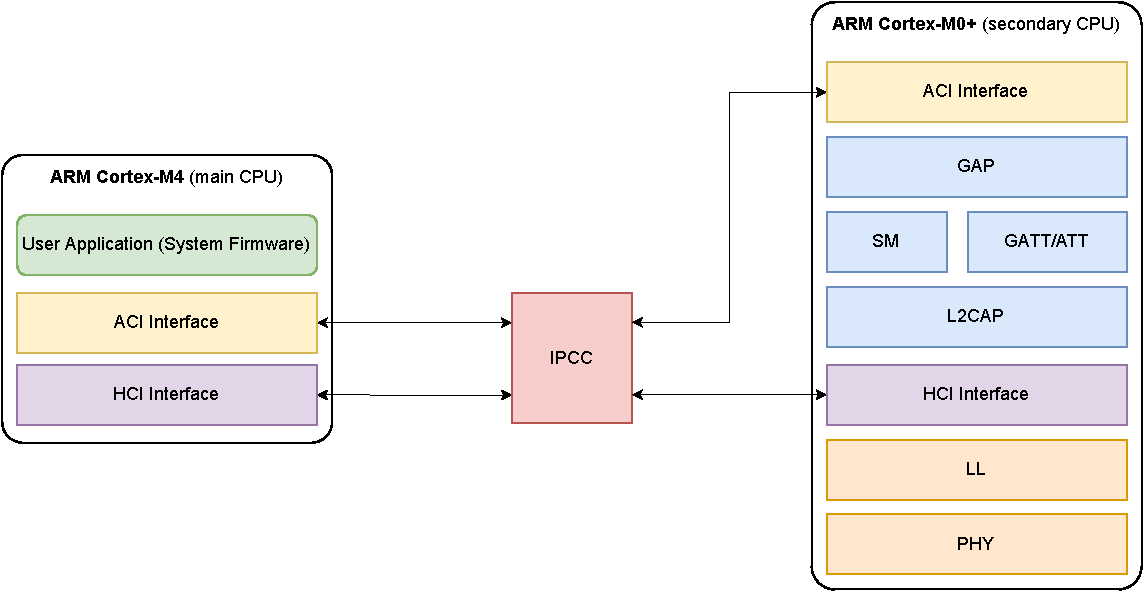
\includegraphics[width=\linewidth]{firmware/firmware_ble_stack_communications}
	\caption{BLE protocol stack and interfaces system implementation. The BLE stack processing and operation is abstracted from the main CPU, which runs the system firmware. The control of the BLE stack in the secondary CPU is performed by the main CPU via commands issued through an inter process communication controller (IPCC) to and from the secondary CPU. This architecture provided by the MCU design allows for system logic in the main CPU to run in parallel to BLE logic in the secondary CPU}
	\label{fig:firmware_ble_stack_communications}
\end{figure}

\subsubsection{BLE protocol stack overview and configuration} \label{sec:ble_stack}

The Bluetooth Low Energy protocol is made up of several layers in an architecture that makes up the BLE protocol stack. In broad terms, the stack can be divided into two parts: \textit{Controller} and \textit{Host}. An overview of the BLE stack layer architecture is provided in \cref{fig:firmware_ble_stack_layers}. A summary of the system BLE stack configuration is provided in \cref{tab:ble_stack_config}.

\begin{figure}[ht]
	\centering
	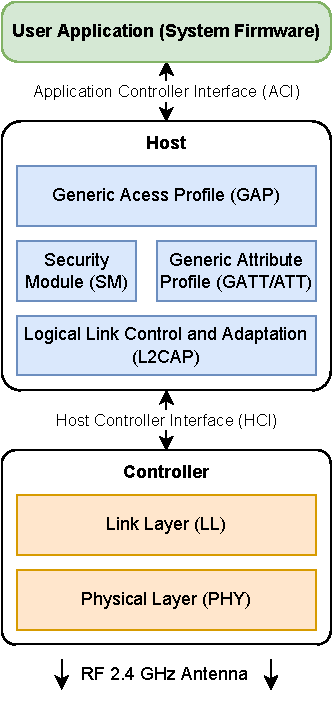
\includegraphics[width=0.3\linewidth]{firmware/firmware_ble_stack_layers}
	\caption{BLE protocol stack layer architecture. On the lowest level, the PHY layer is connected to a 2.4 GHz antenna. On the highest level, control of the BLE link is performed by the user application through the ACI. The \textit{Host} and \textit{Controller} communicate via the HCI.}
	\label{fig:firmware_ble_stack_layers}
\end{figure}

\paragraph{Host}

The \textit{Host} is the higher level part of the stack and is made up of software layers. It includes several protocols itself: \textit{Logical Link Control and Adaptation Protocol} (L2CAP), \textit{Generic Attribute Profile} or \textit{Attribute Protocol} (GATT/ATT), \textit{Security Module} (SM) and \textit{Generic Access Profile} (GAP).

\paragraph{GAP}
This protocol manages device connections, and the discovery of the capabilities of a device when a connection is established. It is based on the role of a device, with respect to its \textit{connection profile}. The roles of a device in BLE can be either \textit{GAP Peripheral} or \textit{GAP Central}. The GAP protocol is used when the devices are in advertisement mode, which is the state of a BLE connection before devices have established a connection. When a BLE connection is yet to be established (advertisement mode) peripherals are visible to central devices and central devices scan for peripherals to issue a connection request. The system is configured such that it acts as a \textit{GAP Peripheral} allowing connections from a data receiving device, the system identifier and device name is set to \textit{SiRadarBLE}.

\paragraph{SM}
This protocol manages encryption and connection security. It is disabled for the configuration of the system, but can be activated by modification of the source code such that the system asks for a password when trying to establish a connection or the data transmission is encrypted in some form [REF].

\paragraph{GATT}
This protocol is used for the transmission and retrieval of information. It is based on the role of a device, with respect to \textit{data flow}. A device in a BLE connection can be either a \textit{GATT Server}, which stores information and provides means for clients to access it, or a \textit{GATT Client}, which accesses data on the remote \textit{GATT Server} through data access operations. These operations are performed on data attribute types called \textit{Characteristics}. \textit{Characteristics} hold a single data value and an arbitrary number of descriptors, which give information about the type of data it represents and the data access configuration. \textit{Notify} and \textit{indicate} are a type of data access operations driven by a subscription of the \textit{GATT Client} to a \textit{Characteristic} of the \textit{GATT Server}. Using \textit{notify} a client can receive data generated by the server. The system implements a single \textit{Characteristic} called \textit{DSP\_DATA} which holds the data generated by the DSP routines in a packet form. This \textit{Characteristic} is only \textit{read} enabled and is configured as a \textit{notification}, such that clients can subscribe to the event of data change and receive new data via the BLE connection. For example: a device wishes to read data sent from another device. In this case, the\textit{GATT Client} who whishes to obtain changing data from a \textit{GATT Server} sends a \textit{notify} command subscribing to changes in the data. As it is a \textit{notify} command, every time the \textit{GATT Server} has new data available, it is sent to the \textit{GATT Client}.

\paragraph{L2CAP}
This protocol manages higher-level protocol multiplexing (i.e. interleaving data from different protocols in the BLE packets \cite{Blel2cap}) and packet segmentation and reassembly operations. The system implements this protocol such that if packets are lost or corrupted they are re-sent through the connection.

\paragraph{Controller}

The \textit{Controller} is the low level part of the stack, including the \textit{Physical Layer} (PHY) with a RF gaussian frequency shift keying (GFSK) transceptor and the \textit{Link Layer} (LL), which handles control of the radio and forward error correction (FEC) of data transmission. The RF radio is used to transmit binary information through specific channels of the industrial, scientific and medical (ISM) radio spectrum. The built-in FEC capabilities allow for basic error corrections due to link interference of distortion. This part of the stack is configured to make use of the high-speed physical link of \SI{2}{\mega\bit\per\second} and \textit{Data Length Extension} which allows packets to contain up to 247 bytes of payload data of 254 total bytes of a BLE packet size.

The communication between \textit{Host} and \textit{Controller} is done via a \textit{Host Controller Interface} (HCI), which is implemented via an inter process communication controller (IPCC) bridging the main CPU and the secondary CPU (\cref{fig:firmware_ble_stack_communications}). The HCI in the system is automatically configured by the MCU and carries BLE connection commands from the main CPU to the secondary CPU, which handles the BLE connection. The HCI is already provided and preconfigured by the manufacturer and its operation is transparent and automatic.

On the other hand, the communication between \textit{Controller} and the system application is performed via the \textit{Application Controller Interface} (ACI). The ACI makes use of the same IPCC used by the HCI. The ACI is formed by a subset of vendor specific commands provided by the manufacturer. These commands encapsulate sets of HCI commands for easier use. ACI commands can be issued to control the BLE connection, such as accepting incoming connection requests or sending a data packet. In the system firmware, ACI commands are used to enable advertisement mode, send data packets and control device disconnection behaviour. The communication between the different parts is depicted in \cref{fig:firmware_ble_stack_communications}.

{\footnotesize\renewcommand*{\arraystretch}{1.4}
\begin{longtable}{@{}>{\raggedright\arraybackslash\bfseries}m{0.25\linewidth}>{\raggedright\arraybackslash}m{0.2\linewidth}>{\raggedright\arraybackslash}m{0.5\linewidth}@{}}
	\toprule
	Parameter & \bfseries{Configuration} & \bfseries{Reason} \\* \midrule
	\endhead
	PHY Data Rate & PHY 2M & Maximises bitrate of the BLE connection to \SI{2}{\mega\bit\per\second}. \\
	LL Data Length Extension & Active & Maximises the amount of data that is sent per packet to 247 bytes.  \\
	L2CAP Packet Retransmission on Error & Active & Must allow retransmission of data if it is not acknowledged by the receiving device, to avoid information loss.  \\
	GATT Role & Server & The system is the device providing data\\
	GATT Characteristic ID & DSP\_DATA & Creation of attribute holding data from DSP routines.  \\
	GATT Characteristic Access & Read and Notify & Data must only be read by a client, subscribing to data change.  \\
	SM Operation & Inactive & Not relevant for system function.\\
	GAP Role & Peripheral & Must allow connection requests from central devices and enable advertisement mode. \\
	GAP Device Name & SiRadarBLE & Must have a unique and descriptive name for identification when central devices are scanning for connections.\\* \bottomrule
	\caption{Summary of the configuration of the BLE protocol stack in the system}
	\label{tab:ble_stack_config}
\end{longtable}}


\subsubsection{Packet configuration and connection control} \label{sec:ble_packet}

A receiving device can connect to the system using the BLE connection. Generated data by the DSP routines is sent through the BLE link encapsulated in BLE data packets. This connection is orchestrated with BLE advertisement packets. The BLE packets are assembled by the \textit{Low Link} (LL) layer of the BLE stack architecture found in the \textit{Controller} stack. The binary information of the BLE packets is transmitted by the PHY GFSK radio.

BLE features exclusively one packet format for all its operating purposes. A BLE packet consists of a header containing the \textit{Preamble} and \textit{Access Address} fields. The \textit{Preamble} field contains information related to transmission codification and link control. The \textit{Access Address} field contains an identification address for the connection between two devices. This prevents collisions between two or more connections happening in the same RF channel. The \textit{Access Address} is assigned after a successful connection of two devices and is formed by a mix of the media access control (MAC) addresses of both central and peripheral devices.

The rest of the BLE packet consists of the protocol data unit (PDU) and a cyclic redundancy check (CRC) field for error detection purposes.

The PDU varies depending on whether the PDU sent is an \textit{Advertising Channel} PDU or a \textit{Data Channel} PDU. A diagram of the contents and structure of both PDUs can be found in \cref{fig:firmware_ble_pdu_structure}.

\begin{figure}[ht]
	\centering
	\subfloat[BLE packet structure containing a \textit{Data Channel} PDU. This PDU contains a L2CAP PDU, which is the PDU generated by the lowest layer of the \textit{Host} stack of the BLE stack architecture. The MIC field is not used in the system implementation. The DSP data payload is contained in the payload field of the L2CAP PDU]{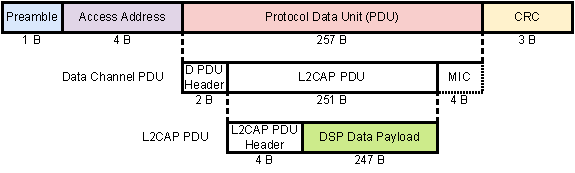
\includegraphics[width=\linewidth]{firmware/firmware_ble_pdu_data} \label{fig:firmware_ble_pdu_data}}\\
	\subfloat[BLE packet structure containing an \textit{Advertising Channel} PDU. This PDU contains a payload with fields holding information about the characteristics of the device connection and services, including the device MAC address. Other fields can be encapsulated in the payload, up to a size limit of 37 bytes, including the 6 bytes of the device address information field ]{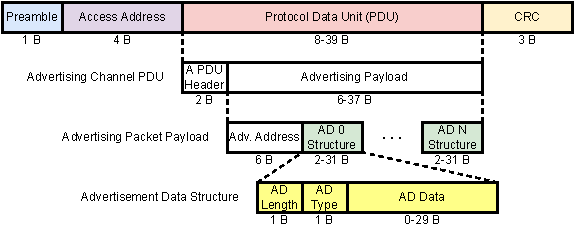
\includegraphics[width=\linewidth]{firmware/firmware_ble_pdu_advertisement} \label{fig:firmware_ble_pdu_advertisement}}
	\caption{Diagram of the BLE packet format with the two different types of PDUs. Note that the BLE packet format is identical for the two PDUs \label{fig:firmware_ble_pdu_structure}}
\end{figure}

In the system BLE configuration, the LL Data Length Extension option is enabled. In this context, each \textit{Data Channel} PDU carries up to 247 bytes of payload data due to protocol overhead of the different layers involved in the BLE stack. A \textit{Data Channel} PDU can optionally carry security information condensed into a message integrity check (MIC) field. However, as the SM is not used in the system, the MIC field contains the null value. The encapsulated DSP data payload location within the BLE packet \textit{Data Channel} PDU can be seen in \cref{fig:firmware_ble_pdu_data}.

\textit{Advertising Channel} PDUs are only sent when the device is in advertisement mode. The system is configured such that it enters this mode by default on a system reset or first boot and in the event of a receiving device disconnecting after being previously connected. \textit{Advertising Channel} PDUs contain information such as the device name (in human readable form, for identification purposes) and the device universal unique identifier (UUID) within the PDU payload. An illustration of the \textit{Advertising Channel} PDUs payloads sent by the system can be found in \cref{fig:firmware_ble_payload_advertisement_system}.

\begin{figure}[ht]
	\centering
	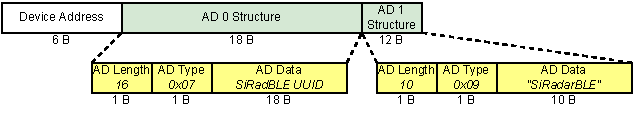
\includegraphics[width=\linewidth]{firmware/firmware_ble_payload_advertisement_system}
	\caption{Diagram of the \textit{Advertising Packet} payloads sent by the system. Each payload contains the system MAC address, and two \textit{Advertisement Data Structures}. The first one contains the universal unique identifier (UUID) of the system and the second one contains the \textit{Complete Local Name} of the system ``\textit{SiRadarBLE}'' in ASCII codification. The name of the system is the visible name that appears in the Bluetooth device selection screen while other devices are scanning for the system
	\label{fig:firmware_ble_payload_advertisement_system}}
\end{figure}

During the system operation, the firmware is programmed such that at a system reset or first boot, the device starts being searchable or discoverable by sending \textit{Advertising Channel} PDUs that BLE devices can receive. After the receiving device which wishes to connect to the system is in range, it issues a connection request that is then accepted by the system. The receiving device then subscribes to the notification of the \textit{DSP\_DATA} characteristic as detailed in \cref{sec:ble_stack}. From that moment onwards, the system sends \textit{Data Channel} PDUs containing DSP data to the connected device until the receiving device disconnects or the system is reset. A temporal sequence diagram of the BLE interaction of the system is shown in \cref{fig:firmware_ble_link_timeline}.


\begin{figure}[!ht]
	\centering
	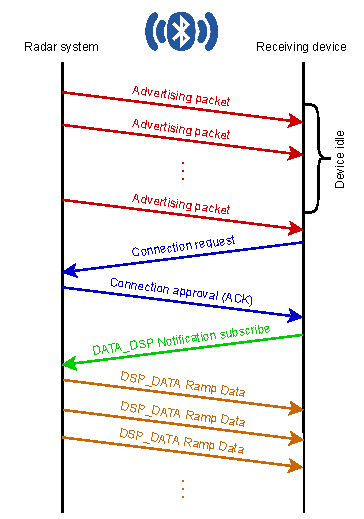
\includegraphics[width=0.6\linewidth]{firmware/firmware_ble_link_timeline}
	\caption{Chronological sequence diagram of the BLE interaction between the system device (radar system) and the data receiving device. The red coloured arrows represent packets sent during the advertisement mode, broadcast to all devices near the radar system. The receiving device idles until it requests a connection to the system. The blue arrows represent connection requests and acknowledgements (ACK). The green arrow represents a \textit{Characteristic} notification subscription. The orange arrows represent data packets
		\label{fig:firmware_ble_link_timeline}}
\end{figure}


\subsection{Data transmission} \label{sec:data_transmission}

As detailed in \cref{sec:ble_packet}, a BLE data packet contains up to 247 bytes of data. It is of interest to organise the generated data by the DSP routines such that the amount of information per packet is maximised. Moreover, the generated data must be stored in such a way that it can be read by the secondary CPU to generate the lower-level bitstream to be sent via the BLE link.

After the sampled data has been processed by the DSP routines described in \cref{sec:dsp_routines}, it must be laid out in chunks of 247 bytes each, so that it can be fitted in independent BLE data packets.

Processed DSP data is found in the $\mathbf{v}$ vector in SRAM memory, as detailed in \cref{sec:adc_tim_config_v_vector}. For every ramp, when the DSP routines finish processing the data, an interrupt is generated and the DMA controller transfers this data to a packet queue for later extraction by the BLE stack processor. The DMA organises the data differently depending if the DSP pipeline has been configured to perform a bin summation for every ramp or the ramp frequency bins are sent as is.

\subsubsection{Packet queuing system}

For packet loss prevention and to ensure packet retransmission in case of error, a packet queuing system has been developed for the radar system, it follows the first in first out (FIFO) principle [REF]. This principle has been chosen as it guarantees that in the event of a packet transmission error, the packet data is still present in the queue for a retransmission attempt while new generated data is not lost or overwritten before being sent.

The queuing system stores the generated packets temporarily in memory until they are extracted by the BLE stack CPU and sent through the BLE link. The FIFO queue has been implemented in the firmware as a driver with data manipulation functions. The FIFO driver source code can be found in Appendix ZZZ. An illustration of the architecture of data storage and extraction of the FIFO queue can be seen in Figure ZZZ.

In the implementation of the system, the FIFO queue has been configured as follows:
\begin{itemize}
	\item Number of items in FIFO queue: 22 BLE data packets. The number of items is maximised as it is the maximum number of packets that can be stored in the capacity of the MCU SRAM [REF].
	\item Item size: 247 bytes. As the queue stores packets, each item size is the same as the packet payload size.
\end{itemize}

For the queue operation, the system stores at all moments a pointer to the queue start and end items. When a new packet has been generated, it is stored in the end pointer address and the pointer is incremented. When a packet is extracted from the queue and sent, the start pointer is incremented. As the FIFO queue size has been set to 22, the system is capable of recovering without discarding new ramp data for a maximum of 21 continuous packet transmission errors.
The storage and retrieval operations of the queue are depicted in Figure ZZZ.

\subsubsection{DSP data packet generation} \label{sec:packet_generation}

To enable asynchronous operation of data transfers in memory, the DSP data is put into the queue via the DMA controller described in \cref{sec:dma}. The utilisation of the queue is distinct according to whether the DSP pipeline performs summation of the frequency bins or whether the bins are transmitted directly.

In this stage, a 16-bit (2-byte) packet ID is appended at the end of every payload. This ID enables the receiving device to identify individual packets and ramps and is generated by incrementing it for every new generated packet. As this number occupies 2 bytes, the usable size of the packet payload is of 245 bytes.

For the case of direct transmission of bins and as every packet holds up to 245 bytes of ramp data, the maximum number of complex bins that can be stored in a packet is 61. This is due to the fact that the real and complex component of a particular bin occupy 16 bits each, for a total of 32 bits (4 bytes), as seen in \cref{fig:firmware_adc_dma_vector}.

The system allows to fit frequency information of multiple ramps into one packet. In the system implementation, the number of complex bins per ramp that are transmitted is set to 20. In this configuration, the frequency bins of three ramps fit into one packet, and as such, the packet is added to the queue as soon as the data of three ramps has been processed by the DSP pipeline. The organisation of the ramp data in each packet using this configuration is depicted in Figure ZZZ. Encapsulating frequency data from multiple ramps has the benefit of increasing the ramp throughput per packet at the cost of decreasing the BLE data packet throughput. Nonetheless, decreasing the BLE data packet throughput is beneficial for reducing the transmission error probability as packets are transmitted more sparsely in time. The relationship between this effects is shown in Figure ZZZ.

The number of bins that are sent per ramp as well as the number of ramps that are encapsulated in each packet can be configured by the user in the source code. It is important to take into account the limitation of the minimum number of frequency bins that contain information about the target range in the application of gait analysis described in ZZZ. This minimum is of ZZZ bins per ramp which is less than the configured 20 bins per ramp of the system. % esto viene de la ecuacion de delta R que depende de la aplicación en la que se utilice el radar. en el caso de gait analysis con 20 bines se obtiene informacion en un rango de x metros que es suficiente para el análisis de la marcha [libro AMIN, RICHARDS]. En el caso de medición de señales vitales, 20 bines también es suficiente para analizar. en nuestro caso basandonos en la ecuacion delta R con 20 bines se obtiene una resolucion en frecuencia de 1.49 m qu es más que suficiente para analizar la marcha de una persona en el caso de gait analysis o el latido de un corazon en el caso de señales vitales.

As the number of sent bins per ramp and the number of ramps that are encapsulated per packet are related, they must be configured correctly. Setting the desired number of ramps encapsulated per packet, it is possible to obtain the maximum number of bins that can be sent per ramp as follows:
\begin{equation}
	N_B = \left\lfloor \frac{P_b}{32 N_R} \right\rfloor
\end{equation}

Where $N_B$ is the number of bins that are sent per ramp, $P_b$ is the payload usable data size in bits (equal to $\SI{245}{B} \cdot \SI{8}{b\per B} = \SI{1960}{b}$), and $N_R$ is the number of encapsulated ramps per packet.

Therefore, a packet is generated and added to the queue every $N_R$ ramps.

\section{Wireless link characterisation} \label{sec:ble_characterisation}

To evaluate the performance of the wireless link based on the Bluetooth Low Energy protocol, a series of measurements have been experimentally performed and their results evaluated. These characterisations of the wireless communication have been performed with the developed system with the hardware implementation described in Section ZZZ and the firmware implementation described in this section.

The results obtained from this characterisation demonstrate that the system is capable of reliably working in real-time with the imposed conditions of the transmission of 20 bins of frequency data per ramp for distances up to 6 metres. For a wireless system whose maximum theoretical distance range of operation is 10 m, it is seen that the requirements for real-time wireless transmission are fulfilled for a comprehensible distance from the radar system.


\subsection{Binary throughput related to BLE antenna distance}

At first instance, the raw binary throughput of the BLE link has been measured. For this measurement the system has been set up to start the transmission of \SI{1}{\kilo\byte} of pre-stored test DSP data. For every measurement, the receiving device has been set up at different distances from the radar system. The distances studied are \SI{25}{\centi\metre}, \SI{50}{\centi\metre} and 1 to 10 \si{\metre} at \SI{1}{\metre} steps. A binary rate measurement is computed by measuring the amount of time it takes to receive the kilobyte of data at the different distances. The results are shown in \cref{fig:firmware_ble_char_bitrate}.

\begin{figure}[ht]
	\centering
	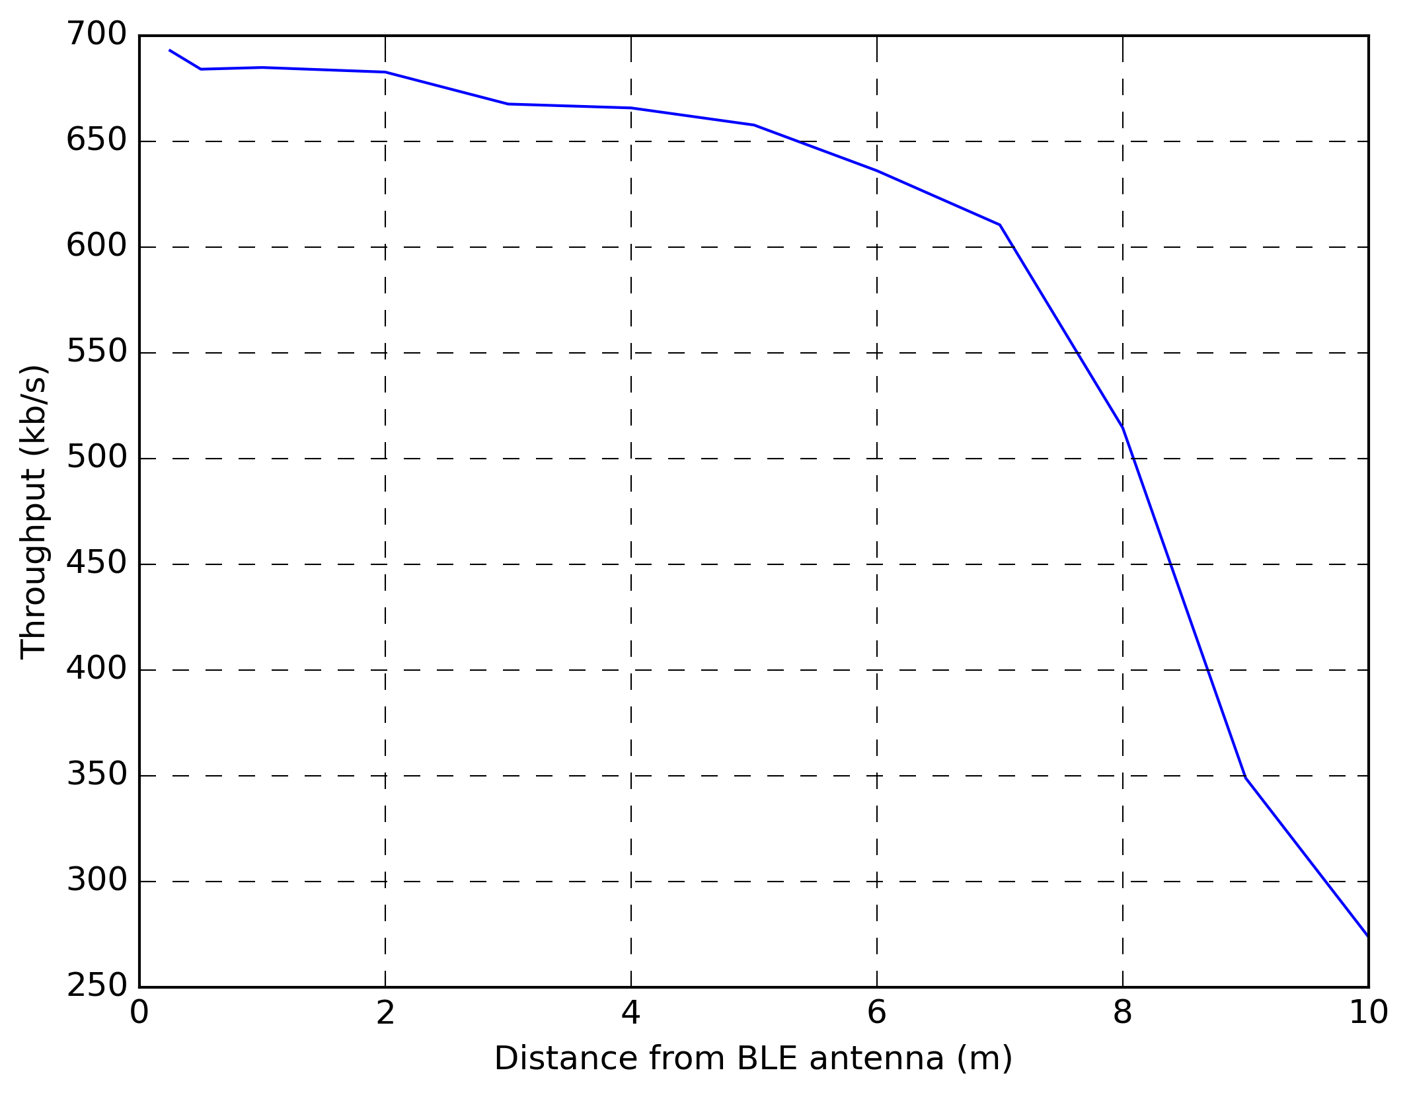
\includegraphics[width=0.6\linewidth]{sucio_graficos/ble/throughput.png}
	\caption{BLE link binary throughput with respect to distance from the BLE antenna. The transmission achieves a bitrate nearing \SI{700}{\kilo\bit\per\second} in distances less than \SI{4}{\meter}. The bitrate is greatly affected in distances greater than \SI{6}{\meter}}
	\label{fig:firmware_ble_char_bitrate}
\end{figure}

The system is capable of delivering around \SI{690}{\kilo\bit\per\second} for a distance to the radar system less than 4 meters, which is very close to the \SI{720}{\kilo\bit\per\second} theoretical maximum bitrate of the protocol, as discussed in \cref{sec:mcu_selection}. The throughput diminishes in an exponential way when the distance is greater than 6 meters, and falling abruptly when reaching 10 meters ---the maximum radio distance for a reliable connection as per the Bluetooth core specification--- [REF].

\subsection{Maximum number of transmitted bins per ramp versus distance} \label{sec:max_number_bins_vs_distance}

A characterisation regarding the bins per ramp that can be sent without any errors has been performed for a set of distances of the receiving device from the BLE antenna. For this part, the complete processing and wireless pipelines are executed and tested. These measurements are performed as follows: 50000 ramps are sampled and processed by the system and sent to the receiving device. The amount of ramps represent around \SI{25}{\second} of ramp data. At every distance, the device is configured to transmit a fixed number of bins per ramp such that no ramp of the 50000 is lost or has a transmission error. To obtain this measurement, the ID of every packet is used to ensure that no missing IDs are found, meaning that all ramps have been successfully received. For this characterisation, retransmitted ramps are considered lost ramps. The distances studied are \SI{25}{\centi\metre}, \SI{50}{\centi\metre} and 1 to 10 \si{\metre} at \SI{1}{\metre} steps. For every distance, the maximum number of bins per ramp that yield no lost ramps is measured. The results are shown in \cref{fig:firmware_ble_char_bins}.

\begin{figure}[ht]
	\centering
	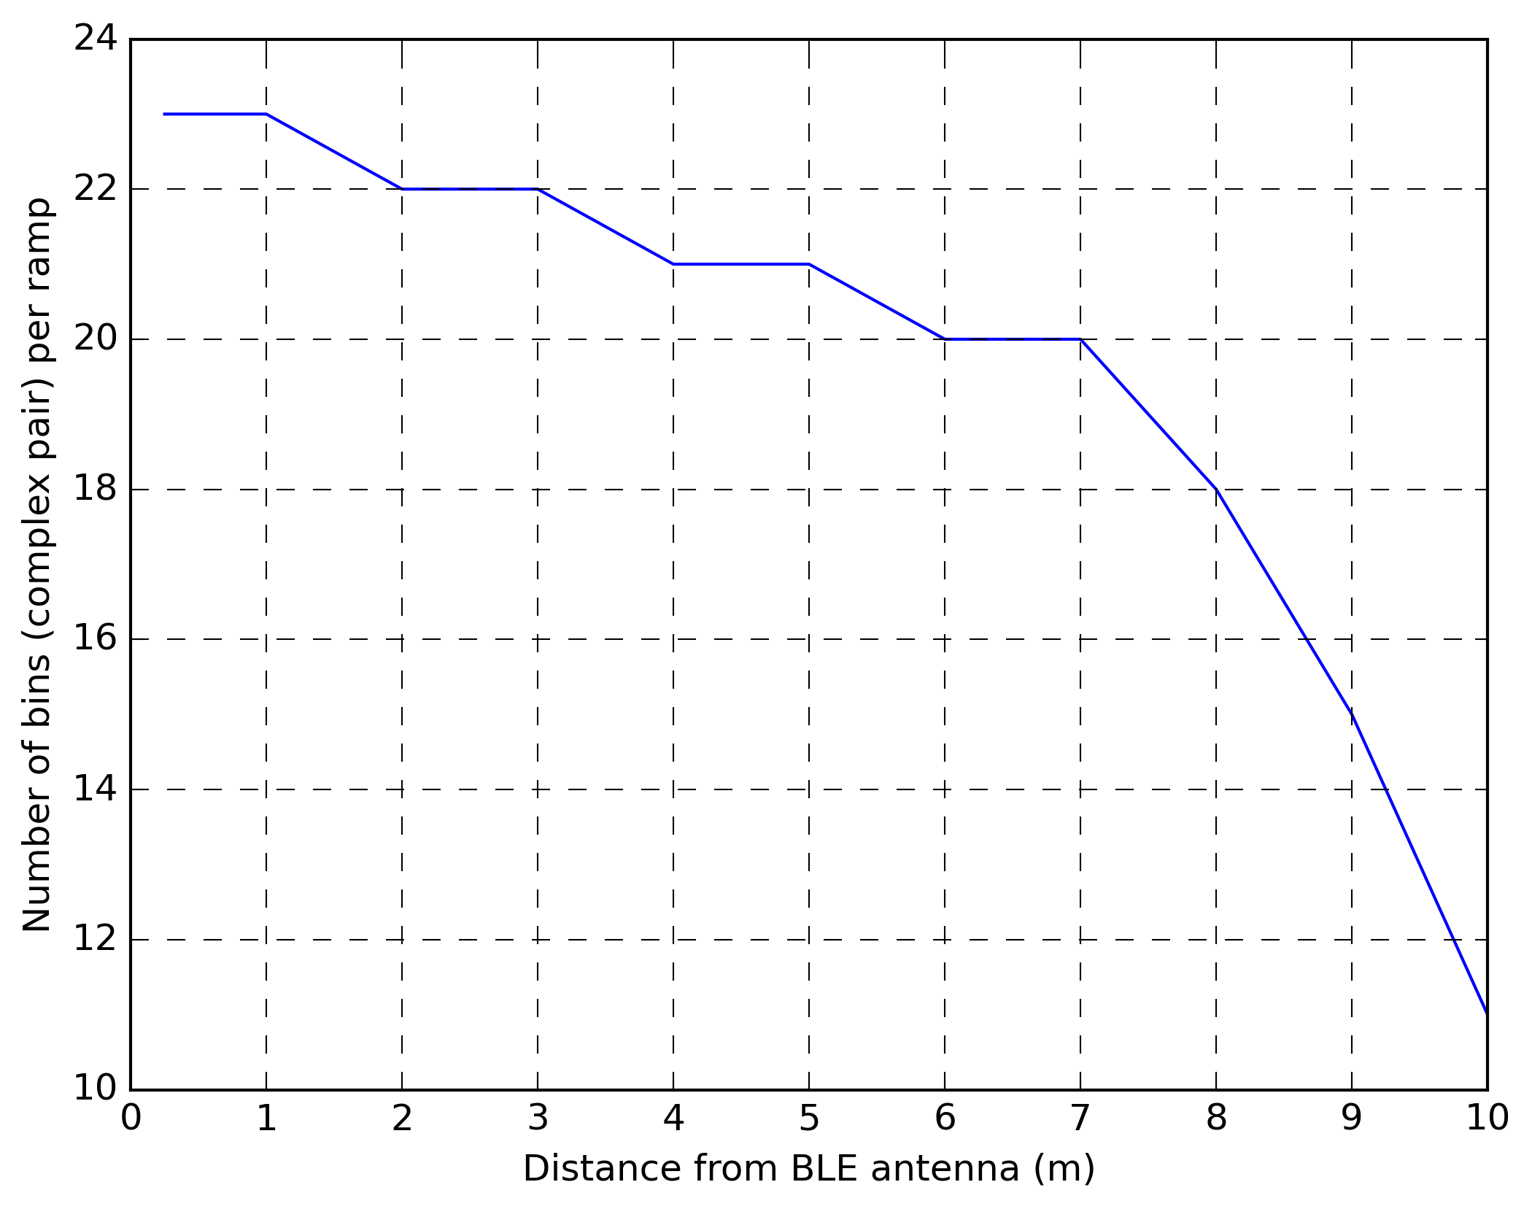
\includegraphics[width=0.6\linewidth]{sucio_graficos/ble/bins_per_ramp.png}
	\caption{Maximum transmitted bins per ramp without ramp loss with respect to distance from the BLE antenna. A maximum of 23 bins per ramp is obtained for the shortest distance. The system configuration of 20 bins per ramp yields no error for distances up to \SI{7}{\metre}. The maximum amount of bins decreases rapidly when the distance is close to \SI{10}{\metre}
	\label{fig:firmware_ble_char_bins}}
\end{figure}

The system is capable of permitting up to 23 bins per ramp for distances up to \SI{1}{\metre} and it has been configured to send 20 bins per ramp, as discussed in \cref{sec:packet_generation}. In this situation, the ramps are sent with no retransmissions or errors in distances up to 7 metres. The maximum number of bins decreases rapidly when approaching the theoretical BLE radio distance limit of 10 metres, described in \cref{sec:mcu_selection}.

\subsection{Bit error ratio (BER)}

A characterisation of the bit error ratio (BER) of the communication has been performed. The system is left transmitting \SI{5}{\mega\bit} of data at different distances of the receiving device from the BLE antenna. The system is configured to transmit incrementing and decrementing (in a loop) 16-bit numbers up to the specified data amount. The distances studied are \SI{25}{\centi\metre}, \SI{50}{\centi\metre} and 1 to 10 \si{\metre} at \SI{1}{\metre} steps. For every distance, the BER is computed as the failed/erroneous bits over transmitted bits, detected as bits out of the expected incremental values. The results are shown in \cref{fig:firmware_ble_char_ber}.

\begin{figure}[ht]
	\centering
	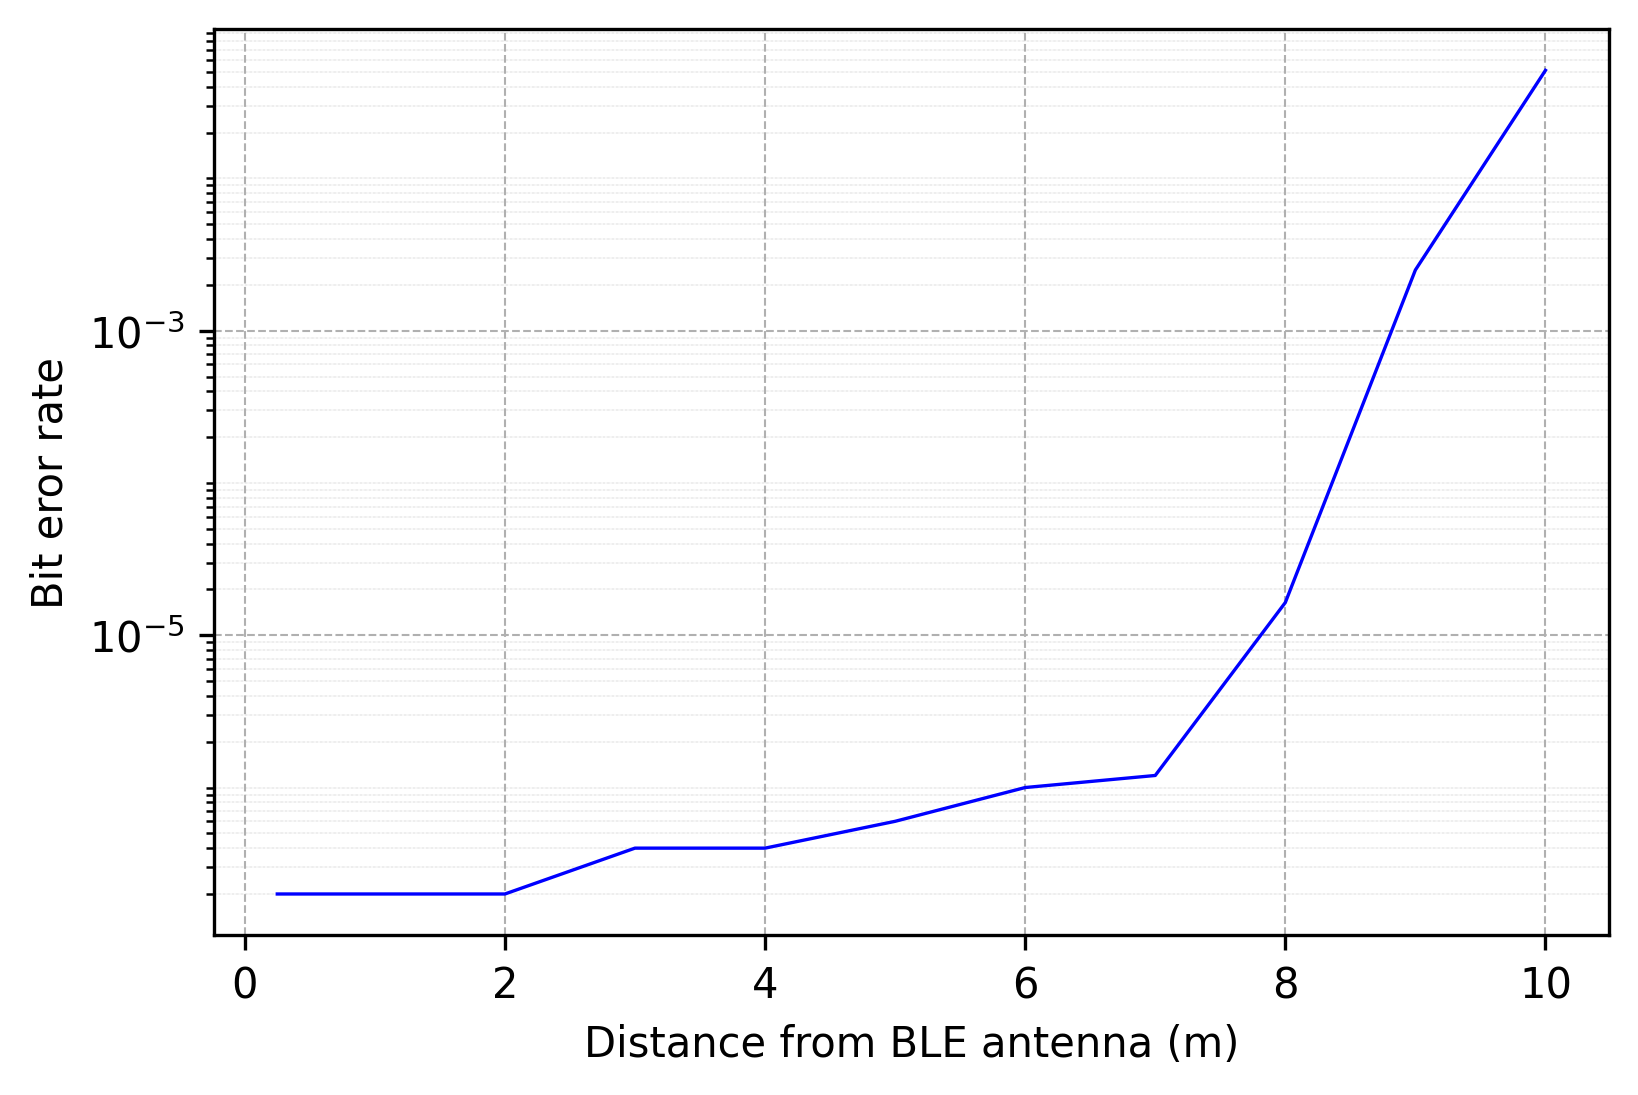
\includegraphics[width=0.6\linewidth]{sucio_graficos/ble/ber.png}
	\caption{Bit error ratio (BER) of the wireless communication link (revisar)}
	\label{fig:firmware_ble_char_ber}
\end{figure}
\subsection{Ramp lost ratio}

A final characterisation has been carried out, in which the ramps that are lost during an extended-time BLE reception are measured with respect to the number of transmitted ramps. This measurement is performed in a range of distances between the receiving device and the BLE antenna. 50000 ramps are sampled and processed by the system and sent to the receiving device. The amount of ramps represent around \SI{25}{\second} of ramp data. For every distance, the same measurement is performed for 20, 10 and 5 bins per ramps. The ratio of successfully received ramps over the total 50000 ramps sent is computed. The results are shown in \cref{fig:firmware_ble_char_rlr}.

\begin{figure}[ht]
	\centering
	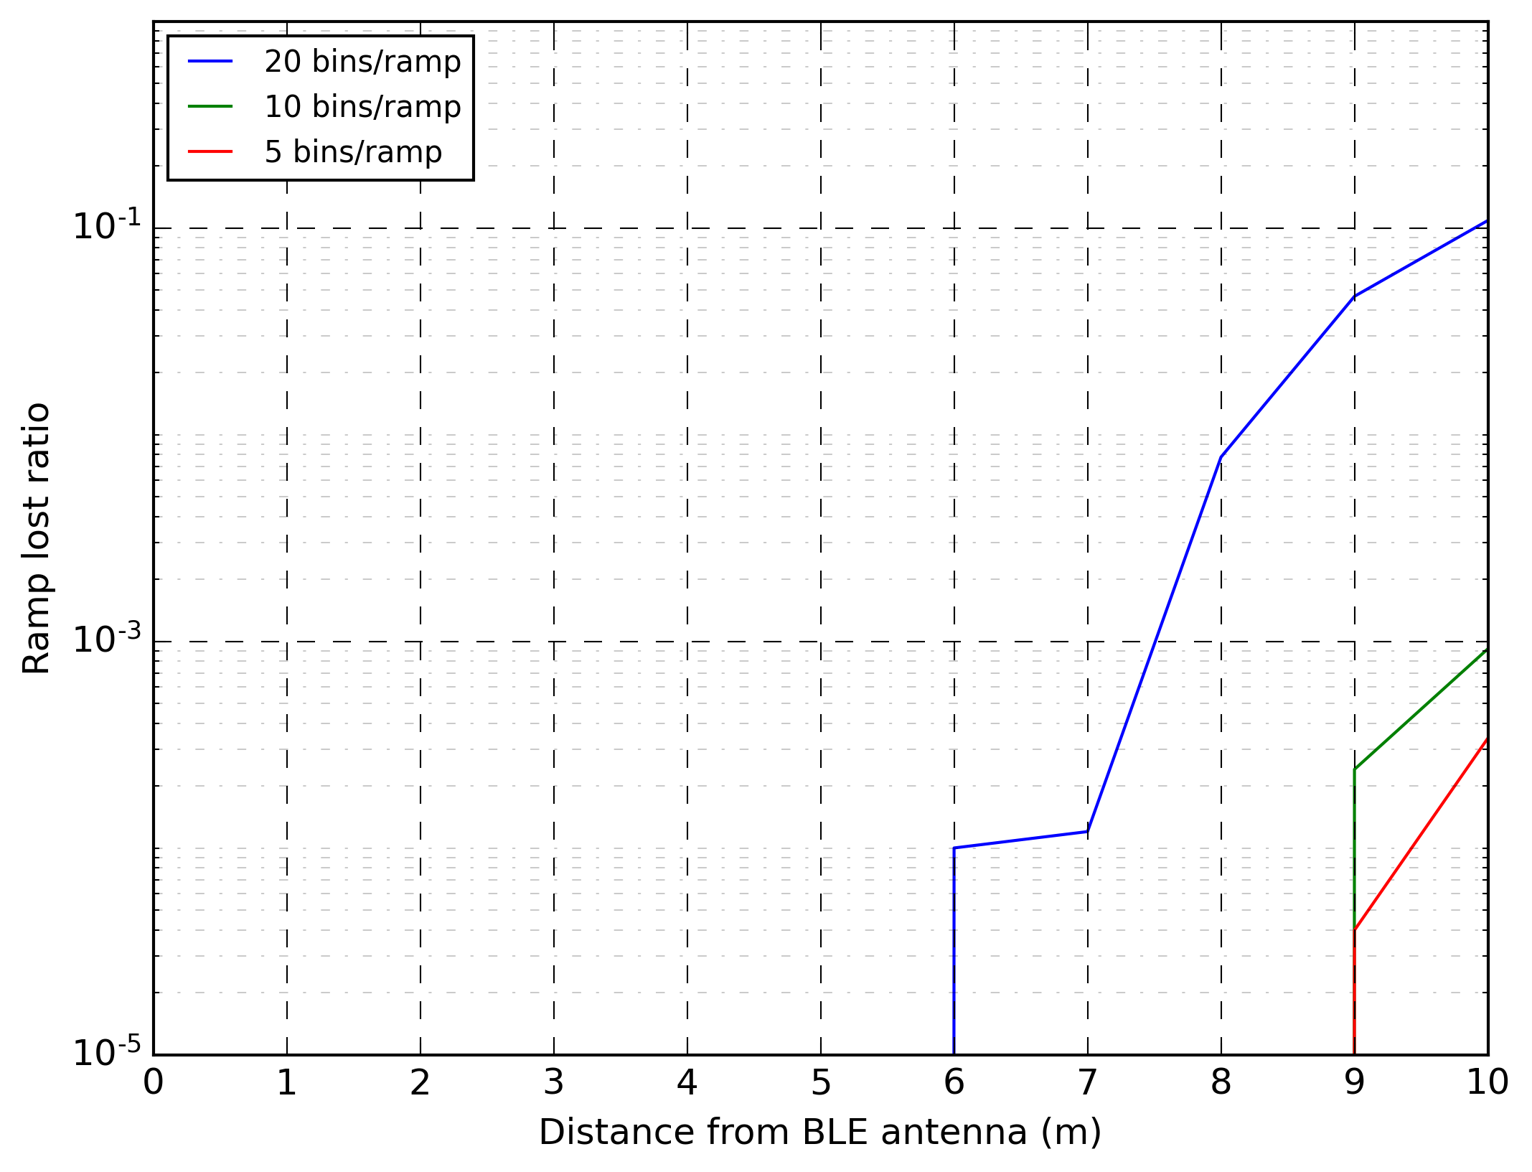
\includegraphics[width=0.6\linewidth]{sucio_graficos/ble/rlr.png}
	\caption{Ramp lost ratio with respect to distance from the BLE antenna. No ramps are lost up to 6 m in all configurations, coinciding with the results obtained in \cref{sec:max_number_bins_vs_distance}. The ratio for 20 bins/ramp begins increasing from 6. The ratio for 10 and 5 bins/ramps is only perceived from a distance starting at 9m. The ordinate axis is represented in a logarithmic scale}
	\label{fig:firmware_ble_char_rlr}
\end{figure}

It is concluded that for distances up to \SI{6}{\metre} no ramps are lost regardless of the amount of ramps that are transmitted. For 10 and 5 ramps per ramp, the transmission is robust for up to \SI{9}{\metre}, close to the theoretical maximum range of Bluetooth operation of \SI{10}{\metre}, as outlined in \cref{sec:mcu_selection}.

% TODO: añadir explicación

% paper del dibujo de range doppler matrix https://www.mdpi.com/2079-9292/9/4/588


